\chapter{Background}

Parton distribution functions (PDFs) bridge the gap between short and long range physics, allowing perturbative Quantum Chromodynamics (QCD) to be applied at the hadronic scale. They embody the incalculable strongly coupled dynamics, and are determined by a comparison of perturbative theory with experiment. Once determined, their form is process-independent and so they can be re-deployed in future calculations. 

This section provides some background to PDFs neccesary for understanding the remainder of this thesis. It is divided in to two main parts, being the necessary physics and the necessary methodology of PDF determination.

To review the physics, we begin by looking at the process of deep inelastic scattering (DIS), and how the na\"ive parton model was developed to explain these experimental observations. Next we look at this in the context of QCD, see how PDFs fit into the picture, and how they evolve with the scale of the physics. Finally we briefly touch on hadron-hadron collisions, which along with DIS constitute the bulk of the processes in modern PDF fits.

To review the methodology we consider the NNPDF fitting strategy, explaining how theory and experiment are used together with neural networks to determine PDFs.

\subsection{Deep inelastic scattering}
For a more in-depth analysis, see Refs. \cite{pinkbook, hm}. In the following background sections we rely heavily on Ref. \cite{nikhefnotes}.

The notion of bombarding matter to uncover its structure has led to many important discoveries in the last hundred or so years, starting with the Geiger-Marsen experiments from 1908-1913 and the subsequent discovery of the atomic nucleus \cite{nucleus}. In the decades following the discovery of the neutron in 1932, nuclei were probed at higher energies, leading to them being understood in terms of ``form factors" which parametrised their electric and magnetic distributions. At this stage it was clear that they were not point-like particles and so a series of important experiments were carried out in the 1960s at the Standford Linear Accelerator (SLAC), involving a high energy beam of charged leptons scattering off a stationary hadronic target. This process is known as Deep Inelastic Scattering (DIS). 

In this section we will consider the example of electrons incident on protons, as shown in Fig. \ref{fig:dis}. In the deep inelastic regime, there is a large momentum transfer, $q=k-k'$, mediated by a virtual photon. The proton, $P$, with initial momentum $p$, fragments into some hadronic state $X$, and the electron starts with energy $E$ and momentum $k$ and ends with energy $E'$ and momentum $k'$. The momentum transfer is large enough that the masses of the proton and electron can be neglected. 

\begin{figure}[H]
\centering
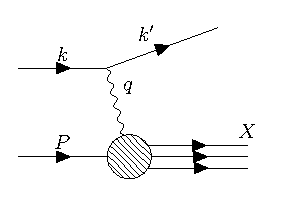
\includegraphics[width=0.7\textwidth]{../diagrams/disdiag.pdf}
\label{fig:dis}
\caption{Deep inelastic scattering}
\end{figure}

It is customary to define some useful variables for help in the analysis, listed in the table below.
\begin{table}[H]
\centering
\begin{tabular}{l|l|l}
  Variable & Definition & Interpretation   \\
 \hline
  $Q^2$ & $- q^2 = -(k-k')^2$   & momentum transfer    \\
  $\nu$ & $p \cdot q = M(E'-E)$ & energy transfer  \\
  $x$   & $\frac{Q^2}{2\nu}$    & scaling parameter \\
  $y$   & $\frac{q \cdot p}{k \cdot p} = 1 - \frac{E'}{E}$ & inelasticity $\in [0,1]$
\end{tabular}
\end{table}
The interaction is made up of a leptonic current (that of the electron) and a hadronic current (the fragmentation of the proton from $P$ to $X$). This means we can express the squared matrix element, $|\mathcal{M}|^2,$ as
\be
\label{eqn:matrixelement}
|\mathcal{M}|^2 = \mathcal{N}_1 \frac{\alpha^2}{q^4} L_{\mu\nu} W^{\mu\nu},
\ee
where $L_{\mu\nu}$ is the leptonic part, determined from perturbative Quantum Electrodynamics (QED), and $W^{\mu\nu}$ is the hadronic part, containing the incalculable strongly coupled dynamics. $\alpha$ is the QED coupling constant and $\mathcal{N}_1$ is a normalisation constant.

From QED, for an unpolarised photon beam in the DIS regime we can use the Feynman rules to write
\bdm
\label{eqn:ltensor}
L_{\mu\nu} = \sum_{spins} \bar{u}(k')\gamma_\mu u(k) \bar{u}(k) \gamma_\nu u(k')
=  Tr \big(\slashed{k'}\gamma_\mu \slashed{k} \gamma_\nu \big)
= \mathcal{N}_2 \bigg( k_\mu k'_\nu + k_\nu k'_\mu -g_{\mu\nu} k\cdot k' \bigg)
= \mathcal{N}_2 \bigg(4 k_\mu k_\nu - 2k_\mu q_\nu - 2 k_\nu q_\mu + g_{\mu \nu} q^2\bigg),
\edm
where in the last line we used the fact that the electron is massless so $
0 = k^{'2} = q^2 + k^2 - 2 q \cdot k \implies q^2 = 2 q \cdot k.$ We have also introduced another constant, $\mathcal{N}_2$.

Finding the hadronic tensor is more difficult because we lack knowledge of the hadronic states $P$ and $X$, so our only constraints are that $W^{\mu\nu}$ is Lorentz-invariant and that the electromagnetic current must be conserved, so $q \cdot W =0$. This allows us to write its general form as
\bdm
\label{eqn:htensor}
W^{\mu\nu}(p,q) = - \bigg(g^{\mu\nu} - \frac{q^\mu q^\nu}{q^2}\bigg) W_1(p,q)
+ \bigg(p^\mu - q^\mu \frac{p \cdot q}{q^2}\bigg) \bigg(p^\nu  - q^\nu \frac{p \cdot q}{q^2} \bigg) W_2 (p, q),
\edm
where $W_1$ and $W_2$ are scalar functions which encapsulate the strong dynamics. These scalar functions are often written as:
\begin{equation}
\begin{split}
F_1(x,Q^2) &= W_1(p,q); \\
F_2(x,Q^2) &= \nu W_2(p,q); \\
F_L(x,Q^2) &= F_2(x,Q^2) - 2x F_1(x,Q^2),
\end{split}
\end{equation}
and are known as the ``structure functions". Often the hadronic tensor is parametrised in terms of $F_2$ and $F_L$, the latter of which is the longitudinal structure function and encapsulates the longitudinal component. 

We can now combine Eqns. \ref{eqn:ltensor} and \ref{eqn:htensor} in Eqn. \ref{eqn:matrixelement}, making use of the fact that due to current conservation $q^\mu L_{\mu \nu} = 0$ to help simplify things. This leads us to the result:
\bdm
\label{eqn:disamplitude}
|\mathcal{M}|^2 = \mathcal{N}_1\mathcal{N}_2^2 \frac{\alpha^2}{q^4} \bigg\{ (-2q^2)W_1(p,q) + \bigg( 4(p \cdot k)^2 - 4 (p \cdot q)(p \cdot k)) \bigg)W_2(p,q) \bigg\}.
\edm

\subsection{The parton model}
Carrying out DIS experiments allows us to measure the structure functions for different values of $x$ and $Q^2$. It transpired that no clear $Q^2$ dependence was observed, and this is known as Bj\"orken scaling \cite{Callan:1973pu}. Because $Q^2$ is the photon's squared momentum, it corresponds to the energy at which the hadron is being probed. The fact that the structure functions are not dependent on this suggests that the interaction is point-like. This led to the formulation of the ``parton model", which described the proton as a composite state made up of point-like particles termed ``partons"\cite{Feynman:1969wa, Feynman:1969ej, Feynman:1973xc}. 

Furthermore, $F_L(x)$ was measured to be 0, known as the Callan-Gross relation \ref{Callan:1968zza, Callan:1973pu}, which suggests that the point-like particles could not absorb longitudinal photons. This fitted in nicely with the quark models developed shortly before \cite{GellMann:1962xb, GellMann:1964nj, Zweig:1964jf, Dothan:1965aa}, which described hadrons in terms of spin-1/2 quarks; spin-1/2 particles cannot interact with longitudinal photons. This was the first experimental evidence for the existence of quarks.

In the DIS regime, $Q^2$ is large and so the virtual photon probes at the short timescale $1/Q$, meaning that the interaction will be effectively instantaneous when compared with the inner proton dynamics which operate at the QCD scale $1/\lambda_{QCD} \sim $ 1 fm.  In the parton model we make the assumption that the partons have only a small momentum transverse to the proton's, and that they are effectively on shell for the interaction ($k^2 \approx 0$). In addition, we consider the process in the infinite momentum frame of the proton, in which it is Lorentz contracted by $M/P$ (a small number), so we can assume the photon will only interact with one parton because it will only traverse a narrow cross-section of the proton. The updated picture is shown in Fig. \ref{fig:disparton}.
\begin{figure}[H]
\centering
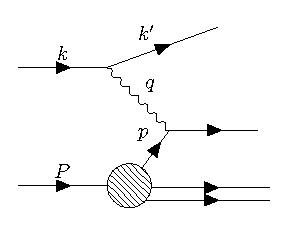
\includegraphics[width=0.7\textwidth]{../diagrams/parton_dis.pdf}
\label{fig:disparton}
\caption{DIS in the parton model. One parton with momentum $p$ interacts with the virtual photon, and the other partons ``spectate".}
\end{figure}

We parametrise the momentum of the interacting parton as $\xi p$, $\xi \in [0,1]$. The parton in the final state has negligible mass so its momentum squared is zero:
\be
\begin{split}
(\xi p+q)^2 &= 0  \\
\implies 2 \xi p \cdot q + q^2 &= 0 \\
\implies 2 \xi p \cdot q - Q^2 &= 0  \\
\implies \xi &= \frac{Q^2}{2p \cdot q} \equiv x.
\end{split}
\ee
This allows us to identify the parton's momentum fraction in this frame with the Bj\"orken $x$ variable.

We can think of the total collection of interactions in terms of a weighted sum over the interactions between the photon and the individual point-like partons, and so can write the proton-level hadronic tensor, $W_{\mu\nu}$ in terms of the parton-level ones, $\hat{W}^q_{\mu\nu}$, as
\be
W_{\mu\nu} = \sum_q  f_q(x) \hat{W}^q_{\mu\nu} \delta(Q^2 - 2xp \cdot q)
= \frac{1}{Q^2} \sum_q  f_q(x) \hat{W}^q_{\mu\nu} \delta(1 - \frac{2xp \cdot q}{Q^2}),
\ee
where $q$ runs over the possible quark flavours and $f_q$ are distributions, with $f_q(x)dx$ giving the probability that in an interaction a parton of flavour $q$ will be found in the momentum range $x \to x +dx$. We call these functions ``parton distribution functions" (PDFs). The delta function appears due to integration over the final phase space of X, and enforces conservation of momentum. Using Eqn \ref{eqn:matrixelement}, we can see that
\be
\label{eqn:ampcomparison}
|\mathcal{M}|^2 = \frac{1}{Q^2} \sum_q  f_q(x) |\mathcal{\hat{M}}_q|^2.
\ee
This means that the total amplitude can be expressed in terms of the partonic amplitudes and the PDFs. If we assume that the partons are massless Dirac particles, we can infer the partonic amplitudes directly from that of electron-muon scattering. In this scenario the electron has a current like Eqn. \ref{eqn:ltensor}, and the muon has the same, but with the substitutions $k \to p$ and $q \to -q$. Once again we can use $q_\mu L^{\mu \nu} =0$ and the expression
\be
|\mathcal{M}_{(e \mu)}|^2 = \mathcal{N}_1 \frac{\alpha^2}{q^4} L^{(e)}_{\mu\nu} L_{(\mu)}^{\mu\nu}
\ee
to show (in the massless limit)
\be 
|\mathcal{M}_{(e \mu)}|^2 = \mathcal{N}_1\mathcal{N}_2^2 \frac{\alpha^2}{q^4} \bigg( 16 (p \cdot k)^2 + 8 q^2 (p \cdot k) + 2 q^4 \bigg).
\ee
Using the symmetry of Fig. \ref{fig:disparton}, we can see this is analogous to $|\mathcal{\hat{M}}_q|^2$ under the substitution $p \to xp$, provided we replace the charge of the electron, $e$, with that of the parton, $e_q$, so that $\alpha \to e_q \alpha$. Making use of the expression $p \cdot k = Q^2/2xy$,
\be 
\begin{split}
|\mathcal{\hat{M}}_q|^2 &= \mathcal{N}_1\mathcal{N}_2^2 \frac{e_q^2 \alpha^2}{q^4} \bigg\{ 4 (2xp \cdot k)^2 + 4 (2 x p\cdot k) q^2 + 2q^4 \bigg\} \\
&= \mathcal{N}_1\mathcal{N}_2^2 \frac{e_q^2 \alpha^2}{Q^4} \bigg\{ 4 \bigg(\frac{Q^2}{y}\bigg)^2 - 4 \bigg(\frac{Q^2}{y}\bigg) Q^2 + 2Q^4 \bigg\} \\ 
&= \mathcal{N}_1\mathcal{N}_2^2 e_q^2 \alpha^2 \bigg\{ 2 + 4 \bigg( \frac{1-y}{y^2} \bigg) \bigg\}.
\end{split}
\ee 
Now we can use this alongside Eqn. \ref{eqn:disamplitude} in  Eqn. \ref{eqn:ampcomparison}, giving us
\be 
\begin{split}
F_1 &\equiv W_1 = \sum_q f_q(x)e_q^2, \\
F_2 &\equiv \nu W_2 = 2x \sum_q f_q(x) e_q^2.
\end{split}
\ee
We see immediately that the Callan-Gross relation, $F_L(x) \equiv F_2(x) - 2x F_1(x) = 0$, is satisfied, as was observed experimentally.

However, it was soon observed that this relation only held in the limit $Q^2 \to \infty$, and that at smaller scales there were so-called ``scaling violations". In order to understand this behaviour it is necessary to revisit the parton model in the light of Quantum Chromodynamics (QCD).

\subsection{Quantum Chromodynamics (QCD)}
QCD is the theory of the strong force. This is responsible for binding together hadrons, and explains the short-range interactions which occur within them. It is a gauge theory where the quark fields are realised as fundamental representations of the $SU(3)$ symmetry group and interactions between them are carried out via gauge bosons termed ``gluons", which are expressed in the adjoint representation \cite{grinstein2006introductory}. 

Quark models showed that the structure of observed hadrons can be explained using the $SU(3)_f$ group alongside the association of quarks with different ``flavours"  \cite{GellMann:1962xb, GellMann:1964nj, Zweig:1964jf, Dothan:1965aa} . The additional $SU(3)_c$ colour symmetry was put forwards in order that the quarks satisfied Fermi-Dirac statistics \cite{Greenberg:1964pe}. Each quark is assigned an additional colour ((anti-)red, green or blue) in such a way that the composite hadrons are colourless. The additional local symmetry is accompanied by eight gauge bosons, the gluons. Colour is the charge of QCD, just as electric charge is for QED. An important difference is that, unlike chargeless photons in QED, the gluons themselves also have colour and this leads to complex self-interactions. 


QCD can be expressed through the Lagrangian
\be
\mathcal{L} = -\frac{1}{4}F_{\mu \nu}^a F^{a \mu \nu} + \bar{q}^i(i \slashed{\mathcal{D}}_i^j - m \delta_i^j) q_j,
\ee
where the covariant derivative is
\be 
\mathcal{D}_\mu \psi(x) = (\partial_\mu -i\sqrt{4 \pi \alpha_s}T^a A_\mu^a) \psi(x) ,
\ee
and the field strength tensor is
\be 
F^a_{\mu \nu} = \partial_\mu A_\nu^a - \partial_\nu A_\mu^a + \sqrt{4 \pi \alpha_s} f^{abc} A_\mu^b A_\nu^c.
\ee
The indices $\mu, \nu$ are spacetime indices, $i, j$ are quark colour indices and $a,b, c$ are gluon colour indices. The first term in the Lagrangian arises from the self-interacting gluons, $A$, and the second term from the quarks, $q$, which obey the Dirac equation. $\alpha_s$ is the strong coupling constant, which dictates the strength of the interaction, and $T^a$ are the eight $SU(3)$ generators. $f^{abc}$ are the SU(3) structure constants. For simplicity we have assumed all quarks have the same mass, $m$. Note that gauge fixing and ghost terms are omitted. For more information see Ref. \cite{pinkbook}.

Colour self-interactions give rise to the important properties of ``confinement" and ``asymptotic freedom". The QCD potential is of the form
\be 
V(r) \sim \frac{\alpha}{r} + kr,
\ee
where the first term drops off with distance like QED, but the second term comes from the self-interactions and means that separating two quarks takes infinite energy. This explains why we have not observed free quarks (``confinement"). Additionally, the QCD colour charge decreases with shorter distances. This means that at very short distances or high energies the quarks become ``free", which is known as ``asymptotic freedom". This crucial fact allows us to applythe tool of perturbation theory in such regimes. 

QCD is subject to divergences in the ultra-violet (high energies) and infra-red (low energies). The former are regulated by renormalisation, which introduces a ``renormalisation scale", $\mu_R$. This is non-physical, and so observables cannot depend on it. This observation leads to a ``renormalisation group equation" (RGE), which can be solved by the introduction of a running coupling, dependent on the scale $Q^2$ (i.e. $\alpha_s \to \alpha_s(Q^2)$), which satisfies
\be
\label{eqn:rge}
Q^2 \frac{\partial \alpha_s}{\partial Q^2} = \beta (\alpha_s),
\ee
The beta function, $\beta(\alpha_s)$, can be expressed perturbatively as an expansion in $\alpha_s$ and is currently known to N$^3$LO.

At one-loop order the solution of this equation is
\be 
\alpha_s(Q^2) = \frac{\alpha_s(\mu_R^2)}{1+ \beta_0 \alpha_s (\mu_R^2) \ln\big(\frac{Q^2}{\mu_R^2}\big)},
\ee
where $\beta_0$ is the first coefficient of the $\beta$ expansion. From this solution we can explicitly see asymptotic freedom because $\alpha_s$ decreases as the energy scale increases. We also see the role of the renormalisation scale in specifying a particular reference value for $\alpha_s$. This solution is not exact because the RGE \ref{eqn:rge} only holds to all orders. Any residual $\mu_R$ dependence characterises the accuracy of our calculation, because going to higher and higher orders should reduce this dependence, eventually to 0.

Quantities are infra-red safe if they do not depend on long-distance physics. This means we can apply perturbation theory because $\alpha_s$ is small enough in the short-distance regime. Unforunately at the partonic level structure functions and cross sections are not infra-red safe. 

\subsection{The QCD improved parton model and factorisation}

In the na\"ive parton model, we did not include any interactions involving gluons; their incorporation leads to the QCD improved parton model. The addition of gluons leads to significant complications, owing to the fact that the interacting quarks are free to emit gluons at some stage before detection (remember the detector is at a long-distance so we cannot ignore the long-distance physics). When these gluons are ``soft" (low energy) or collinear to one of the partons we run into IR divergences. This situation is equivalent to the internal propagator quark going on-shell, or in other words there is a large time separation between the partonic interaction and the gluon emission. The observed violation of Bj\"orken scaling has its origins in interactions with gluons. In IR-safe observables the soft and collinear divergences exactly canel \cite{Kinoshita:1962ur, Lee:1964is}, but for other cases we need a way of dealing with the disparate short- and long- scale physics. 

This is done using the factorisation theorem \ref{Collins:1989gx}, which allows us to factorise the incalculable long-distance physics into the PDFs, meaning we are able to use perturbative QCD as a predictive theory. The PDFs are then non-perturbative, meaning we must obtain them from experiments, but they are universal quantities and so once determined can be applied everywhere, much like the coupling constants. This process introduces the artificial ``factorisation scale", $\mu_F$, in addition to the renormalisation scale. The factorisation scale separates the short- and long- distance physics; loosely, if a parton's transverse momentum is less than $\mu_F$ it is considered part of the hadron and is factored into the PDFs, otherwise it is seen as taking part in the hard scattering process, and will appear in the partonic cross section.

\begin{figure}[H]
\centering
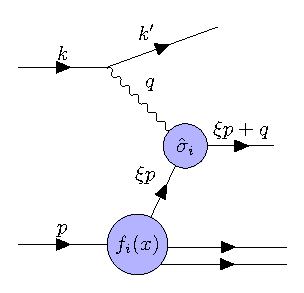
\includegraphics[width=0.7\textwidth]{../diagrams/improvedparton_dis.pdf}
\label{fig:improvedparton}
\caption{Factorisation and the QCD improved parton model}
\end{figure}


We can write a DIS cross section as
\be
\label{eqn:disfact}
\sigma^{DIS} = \sum_i \int dx f_i(x, \mu_F^2) \hat{\sigma}_i \bigg(x, \frac{Q^2}{\mu_F^2} \bigg),
\ee
corresponding to Fig \ref{fig:improvedparton}. 

We can see how this works in practice by considering the case where a quark emits a gluon before interaction with the photon, such as in Fig. \ref{fig:scalingviolation}. Here the parent parton, with fraction $y$ of the proton's momentum, emits a gluon giving rise to a daughter parton with a fraction $z$ of the parent hadron's momentum. We can see that $z = x/y$.

\begin{figure}[H]
\centering
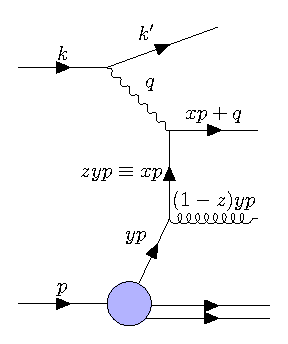
\includegraphics[width=0.7\textwidth]{../diagrams/scalingviolation.pdf}
\label{fig:scalingviolation}
\caption{A quark radiating a gluon before interacting.}
\end{figure}

It transpires (see Ref. \cite{hm} for the derivation) that the structure function $F_2$ can be expressed as
\begin{dmath}
\label{eqn:stfn}
\frac{F_2(x,Q^2)}{x} = \sum_i e_i^2 \int_x^1 \frac{dy}{y} f_i(y) \bigg[ \delta \bigg( 1- \frac{x}{y} \bigg) + \frac{\alpha_s}{2 \pi} \mathcal{P}_{qq} \bigg( \frac{x}{y} \bigg) \ln \bigg( \frac{Q^2}{m^2} \bigg) \bigg].
\end{dmath}
$m$ is a cutoff introduced to regularise the collinear divergence and you can see that as $m \to 0$ the structure function diverges. A divergence also occurs for $(1-z) \to 0$, and this is a soft divergence because it corresponds to the gluon being emitted with zero momentum. The quantity $\mathcal{P}_{qq}$ is the quark-quark ``splitting function", detailing the probability that a quark emits a gluon leaving a daughter quark with fraction $z$ of the parent's momentum. In the $\overline{MS}$ renormalisation scheme this has the form
\be 
\mathcal{P}_{qq} = \frac{4}{3} \bigg( \frac{1+z^2}{1-z} \bigg).
\ee
We want an expression which is free from the soft and collinear divergences. We can proceed by defining
\be 
\mathcal{I}^i_{qq}(x) \equiv \frac{\alpha_s}{2 \pi} \int_x^1 \frac{dy}{y} f_i(y)\mathcal{P}_{qq} \bigg( \frac{x}{y} \bigg),
\ee
and separating \ref{eq:stfn} into a singular part and a calculable part, like
\begin{dmath}
\frac{F_2(x,Q^2)}{x} = \sum_i e_i^2 \bigg[ f_i(x) + \mathcal{I}^i_{qq}(x)  \ln \bigg( \frac{\mu_F^2}{m^2} \bigg) + \mathcal{I}^i_{qq}(x)  \ln \bigg( \frac{Q^2}{\mu_F^2} \bigg) \bigg].
\end{dmath}
Notice we introduced the artificial factorisation scale, $\mu_F$, to do this. Grouping the singular terms together as
\be
f_i(x, \mu_F^2) =  f_i(x) + \mathcal{I}^i_{qq}(x)  \ln \bigg( \frac{\mu_F^2}{m^2} \bigg),
\ee
we have factorised the divergences into the PDF $f_i(x)$, giving a new PDF, $f_i(x, \mu_F^2)$ , which also depends on $\mu_F$.
and noting that at leading order $f_i(y) = f_i(y, \mu_F^2)$, we are able to write
\begin{dmath}
\frac{F_2(x,Q^2)}{x} = \sum_i e_i^2 \bigg[ f_i(x, \mu_F^2) + \frac{\alpha_s}{2 \pi} \int_x^1 \frac{dy}{y} f_i(y, \mu_F^2)\mathcal{P}_{qq} \bigg( \frac{x}{y} \bigg) \ln \bigg( \frac{Q^2}{\mu_F^2} \bigg) \bigg]+ \mathcal{O}(\alpha_s^2).
\end{dmath}
We know that $F_2$ is an observable quantity and thus should be independent of $\mu_F$, leading to a RGE:
\be
\begin{split}
\frac{1}{e_i^2x} \frac{\partial F_2(x,Q^2)}{\partial \ln \mu_F^2} &= \frac{\partial f_i(x,\mu_F^2)}{\partial \ln \mu_F^2} \\ &+ \frac{\alpha_s}{2 \pi} \int_x^1 \frac{dy}{y} \bigg( \frac{\partial f_i(y,\mu_F^2)}{\partial \ln \mu_F^2}\ln \bigg( \frac{Q^2}{\mu_F^2} \bigg) -  f_i(y, \mu_F^2) \bigg)\mathcal{P}_{qq} \bigg( \frac{x}{y} \bigg)\\ &= 0.
\end{split}
\ee
This can be further simplified by noting that $\frac{\partial f_i(y,\mu_F^2)}{\partial \ln \mu_F^2}$ is of $\mathcal{O}(\alpha_s^2)$, and so
\be
\frac{\partial f_i(x,\mu_F^2)}{\partial \ln \mu_F^2}  =  \frac{\alpha_s}{2 \pi} \int_x^1 \frac{dy}{y} f_i(y, \mu_F^2)\mathcal{P}_{qq} \bigg( \frac{x}{y} \bigg).
\ee
This equation describes the evolution of the newly defined PDFs with scale, a product of the factorisation of the divergences into them. In practice this equation is solved numerically. 

When we also include the gluon as a parton, we open ourselves up to more splitting possibilities (e.g. gluon $\to$ quark and gluon $\to$ gluon), and this result generalises to a set of coupled differential equations known as the DGLAP equations~\cite{jr:altarelli, jr:dokshitzer,jr:gribov}:
\be 
\label{eqn:DGLAP}
\frac{\partial f_i}{ \partial \ln \mu_F^2} = \sum_i \frac{\alpha_s}{2 \pi} \mathcal{P}_{ij} \otimes f_j,
\ee
where we have used the Mellin convolution, defined
\be 
\mathcal{P} \otimes f \equiv \int_x^1 \frac{dy}{y} \mathcal{P} \bigg( \frac{x}{y} \bigg)f(y, \mu_F^2),
\ee
and the index $i$ runs from $-n_f$ to $n_f$ (where $n_f$ is the number of flavours), with the negative indices referring to the antiquarks, 0 to the gluon and the positive ones to the quarks.

\subsection{Hadroproduction}

At the LHC most processes involve the interaction of two protons. Hadron-hadron collisions can be approached in much the same way as DIS, but instead the process is like in Fig. \ref{fig:hadroproduction}. Because two protons are involved the expression for the cross section is the natural extension of the DIS case (\ref{eq:disfact}):
\be
\sigma = \sum_{i,j} \int dx_1 dx_2 f_i(x_1, \mu_F^2) f_j(x_2, \mu_F^2) \hat{\sigma}_{ij}\bigg(x_1, x_2, \frac{Q^2}{\mu_F^2},...\bigg).
\ee

\begin{figure}[H]
\centering
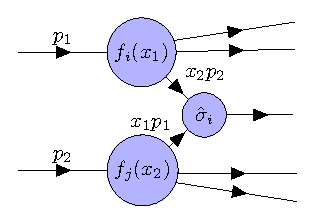
\includegraphics[width=0.7\textwidth]{../diagrams/hadroproduction.pdf}
\label{fig:hadroproduction}
\caption{Factorisation in hadron-hadron collisions.}
\end{figure}

Write about higher order corrections and factorisation!

\subsection{Sum rules}

Although PDFs may seem at first sight to be totally unknown there are some theoretical observations which
we can use to constrain their form.
These are known as the ``sum rules''~\cite{ob:ellis}. Intuitively, adding up all the momenta of the partons must equal the
momentum of the proton. This enforces the condition

\beq
  \int_0^1 dx \sum_i x f_i(x,Q^2) = 1.
\eeq

The other thing we know about the
proton is that it is made up of two up and one down (and no strange)
``valence'' quarks. Any other quarks must be pair-produced from the sea, and
therefore come with an antiquark of the same flavour. So we can normalise the PDFs using the expressions: 

\begin{subequations}
 \beq
   \int_0^1 dx \big( f_u - f_{\bar{u}} \big) = 2;
 \eeq
 \beq
   \int_0^1 dx \big( f_d - f_{\bar{d}} \big) = 1;
 \eeq
 \beq
   \int_0^1 dx \big( f_q - f_{\bar{q}} \big) = 0, \qquad q = s, c, t, b.
 \eeq
\end{subequations}

Note that these conditions require that the PDFs are integrable. 


\section{Determining PDFs}

In this section we review the necessary background for PDF determination within the NNPDF \cite{nnpdf} framework. First we touch on the experimental and theoretical inputs to PDF fits, then we summarise the NNPDF fitting strategy, and finally we detail information on neural networks specific to this context.

\subsection{Experimental and theoretical input}


NNPDF uses a variety of experimental data from a number of particle colliders, including those based at CERN \cite{cern} and Fermilab \cite{fermilab}. These are observables such as cross sections, differential cross sections and structure functions. Fig. \ref{data} is a plot of the $(x,Q^2)$ range spanned by the datasets in the latest NNPDF3.1~\cite{Ball:2017nwa} release. The majority of the data are from DIS processes, which are crucial in determining PDF functional form, but in recent years increasingly more LHC collider data has been added including $t\bar{t}$ production, high energy jets and single top production \cite{Nocera:2019wyk}. For a full review of the data, see Ref. \ref{Ball:2017nwa}.

\begin{figure}
\centering
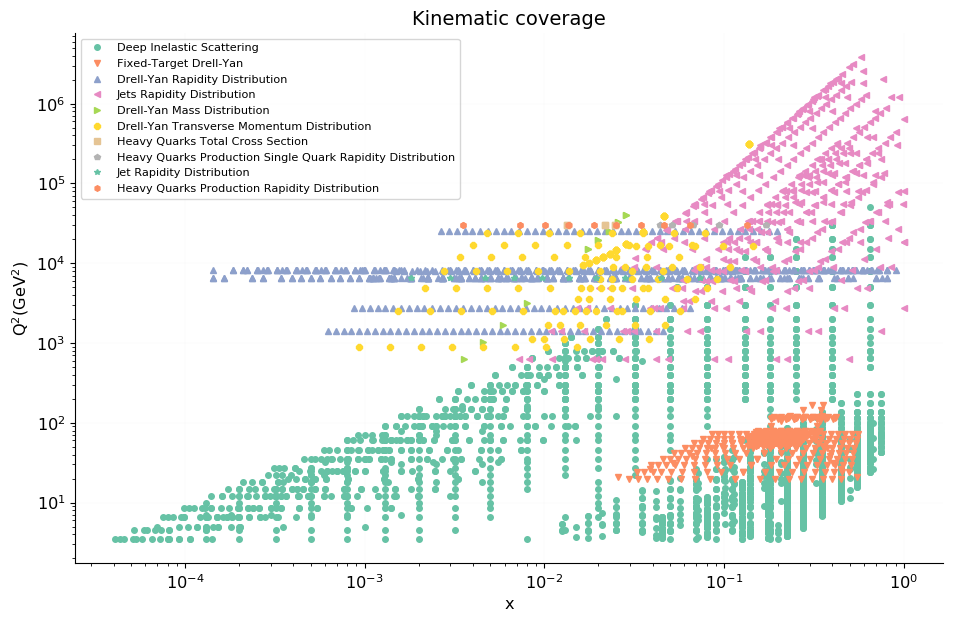
\includegraphics[width=15cm]{background/NNPDF31_nlo_as_0118_1000_markers0_fitcontext_plot_xq2.png}
\caption{Plot of the $(x,Q^2)$ range spanned by data included in the latest NNPDF3.1 NLO fit.}
\label{data}
\end{figure}

Theoretical predictions of the corresponding parton-level observables are computed using external codes such as \texttt{MCFM}~\cite{jr:mcfm}, \texttt{aMC@NLO}~\cite{Alwall:2014hca}, \texttt{DYNNLO}~\cite{Catani:2009sm}, \texttt{FEWZ}~\cite{Gavin:2010az} and \texttt{NLOjet++}~\cite{Catani:1996vz}. These are converted to higher orders of perturbation theory as necessary using QCD and electroweak correction (``$k$'') factors. They are then combined with DGLAP evolution kernels, which evolve PDFs from an initial reference energy scale to the energy scale of each experiment using the DGLAP equations (Eqn. \ref{eqn:DGLAP}). 


\subsection{Experimental uncertainties}
\label{sec:expuncs}

Experimental uncertainties are described using a covaraince matrix, $C_{ij}$, which gives the uncertainties and correlations between each of the data points $i,j = 1,...,N_{dat}$. It encapsulates the total breakdown of errors, $\sigma$, and can be constructed using uncorrelated errors ($\sigma_i^{uncorr}$), and  additive ($\sigma_{i,a}$) and multiplicative  ($\sigma_{i,m}$) correlated systematic errors (more on these below):
\beq
  C_{ij} = \delta_{ij}\sigma_i^{uncorr}\sigma_j^{uncorr} + \sum_a^{add.}\sigma_{i,a}\sigma_{j,a} +
  \bigg( \sum_m^{mult.}\sigma_{i,m}\sigma_{j,m} \bigg) D_i D_j,
\label{eq:expcov}
\eeq
where $D_i$ are the experimental data values.

Structurally, the uncorrelated statistical uncertainties appear down the diagonal and these are what we would recognise intuitively as the statistical error ``on a data point". However, correlated
systematic uncertainties can also appear on the off-diagonals. Correlated uncertaintes include
those which link multiple data points, for example systematic uncertainties from a particular
detector which will affect all of its data in a similar way.

Systematic uncertainties further divide into two types, ``additive'' and ``multiplicative''.
Additive systematics are perhaps a more familiar type of error, and are independent of the
datapoint values themselves. On the other hand,  multiplicative systematics depend on the measured values. In the context of particle physics 
experiments, a common example is total detector luminosity. This is because recorded cross
sections are dependent on the luminosity of the detector; a higher luminosity means more
collisions will take place so the measured cross section will be greater.

Fig. \ref{fig:expcovmat} is an example of an experimental covariance matrix for data included in an NNPDF fit. The data are grouped according to what type of process the interaction belongs to (DIS charged current (CC) and neutral current (NC), Drell-Yan (DY), jets and top production). Systematic correlations within experiments are responsible for off-diagonal contributions, and these are mostly positive correlations but there is some anticorrelated behaviour in DIS CC, as a result of data in different kinematic regimes. 

\begin{figure}
\centering
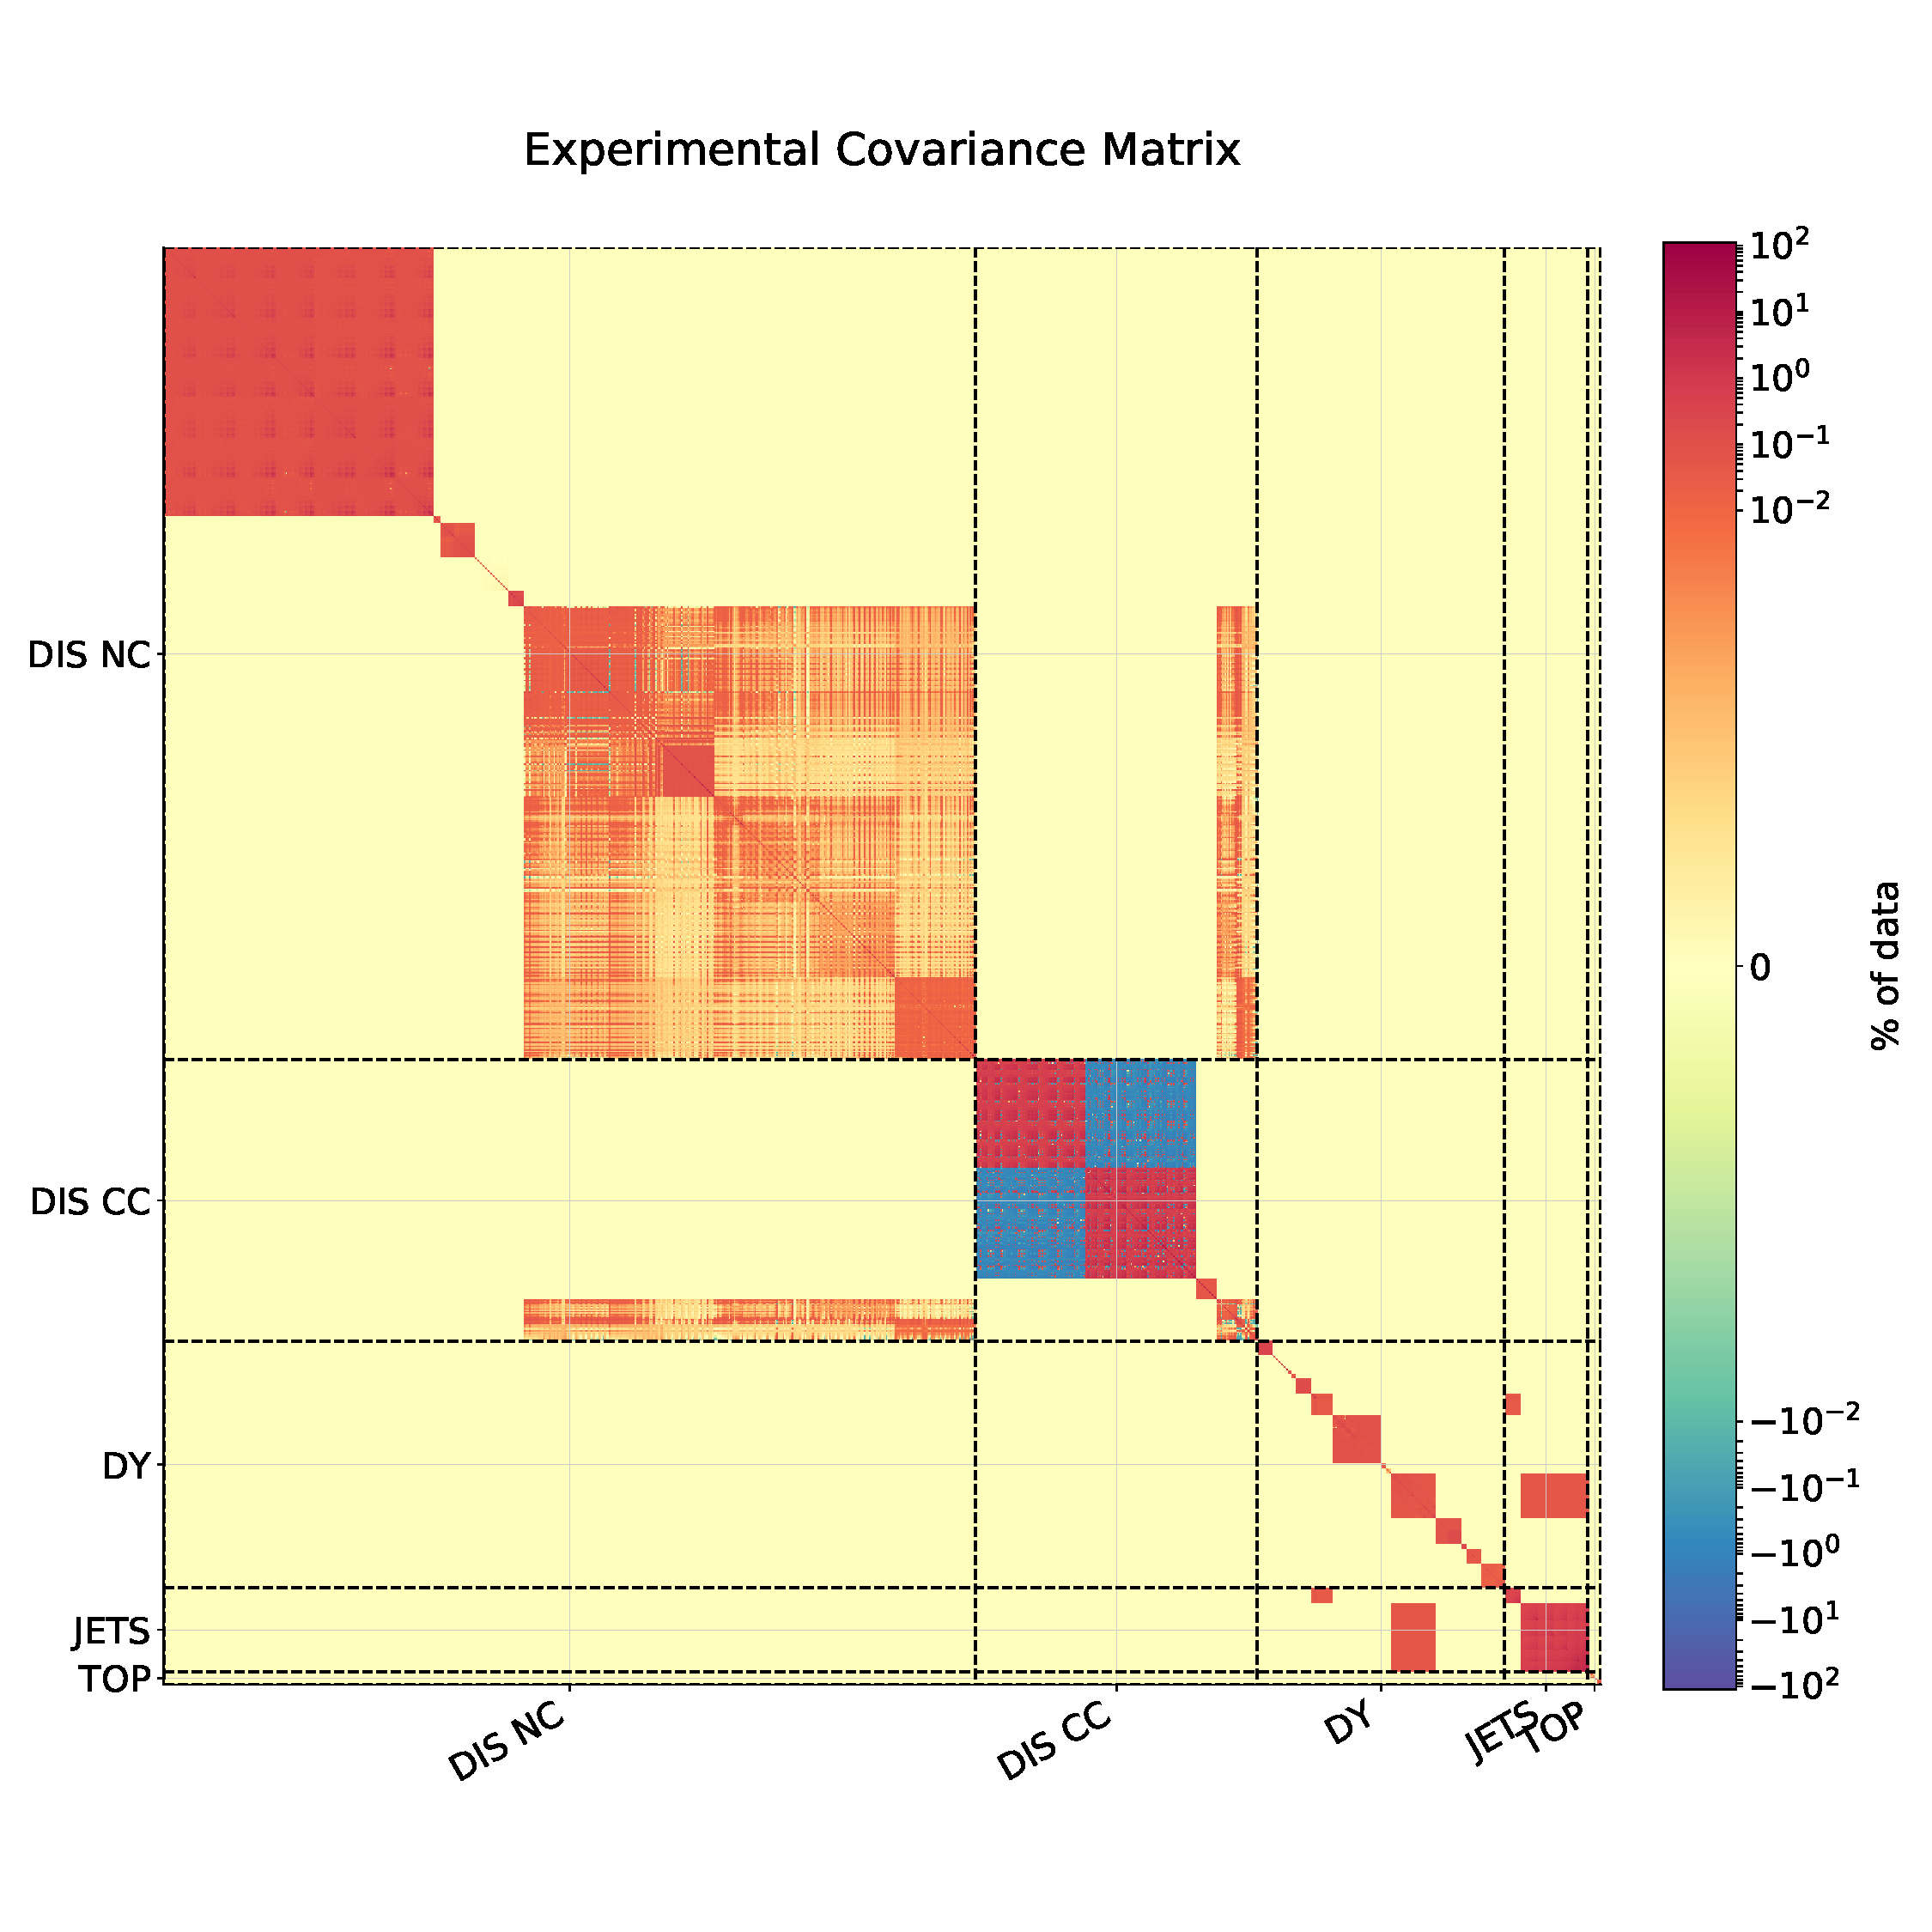
\includegraphics[width=15cm]{background/exp_covmat.pdf}
\caption{An example of an experimental covariance matrix for data included in an NNPDF fit. The data are grouped according to what type of process the interaction belongs to (DIS charged current (CC) and neutral current (NC), Drell-Yan (DY), jets and top production).}
\label{fig:expcovmat}
\end{figure}

The covariance matrix can be used to define the $\chi^2$ figure of merit, 
\be
\label{eqn:chi2}
\chi^2 = \frac{1}{N_{dat}} (D_i-T_i) C_{ij}^{-1} (D_j-T_j),
\ee
which measures the goodness of fit between the experimental data $D_i$ with associated error breakdown $C_{ij}$, and theory predictions $T_i$. In practice, this definition is subject to d'Agostini bias \cite{DAgostini:1993arp} due to the presence of normalisation uncertainties. To avoid this, NNPDF employ the iterative $t0$ procedure \cite{Ball:2009qv} whereby $D_i$ in Eqn. \ref{eqn:expcov} are replaced initially with the predictions from a baseline fit, and the covariance matrix is iterated concurrently with preprocessing. 


\subsection{NNPDF fitting strategy}

There are a number of groups currently active in carrying out PDF fits including MSTW~\cite{Martin:2009bu}, CTEQ~\cite{Dulat:2015mca}, NNPDF~\cite{nnpdf}, HERAPDF/xFitter~\cite{CooperSarkar:2011aa} and ABM~\cite{Alekhin:2013nda}.

The work in this thesis has been carried out in the framework developed by the NNPDF collaboration, so we will concentrate on this fitting strategy. There are two main features which differ from other fitting collaborations'~\cite{Forte:2002fg}. These are:
\begin{enumerate}
\item  The use of Monte Carlo approach to error analysis;
    \item  Fitting using artificial neural networks.
\end{enumerate}

In the following sections we will provide an overview of these aspects, which can be found in more detail in Refs. \cite{Ball:2010de, Ball:2012cx, Ball:2017nwa}.
\subsection{Monte Carlo approach}

The uncertainties in the functional form of PDFs come as a direct consequence of the uncertainties in the experimental and theoretical input. In order to propagate experimental uncertainties through to the PDFs, NNPDF represent the experimental data (central values and uncertainty distribution) as a Monte Carlo ensemble. This is a set of $N_{rep}$ Monte Carlo ``replicas" which, given high enough replica number, have a mean value equal to the data central value and covariance equal to the experimental covariance. Fig. \ref{fig:MC} is a schematic illustrating the generation of these ``pseudodata", $D^{(k)}$, $k=1,...,N_{rep}$.
\begin{figure}
\centering
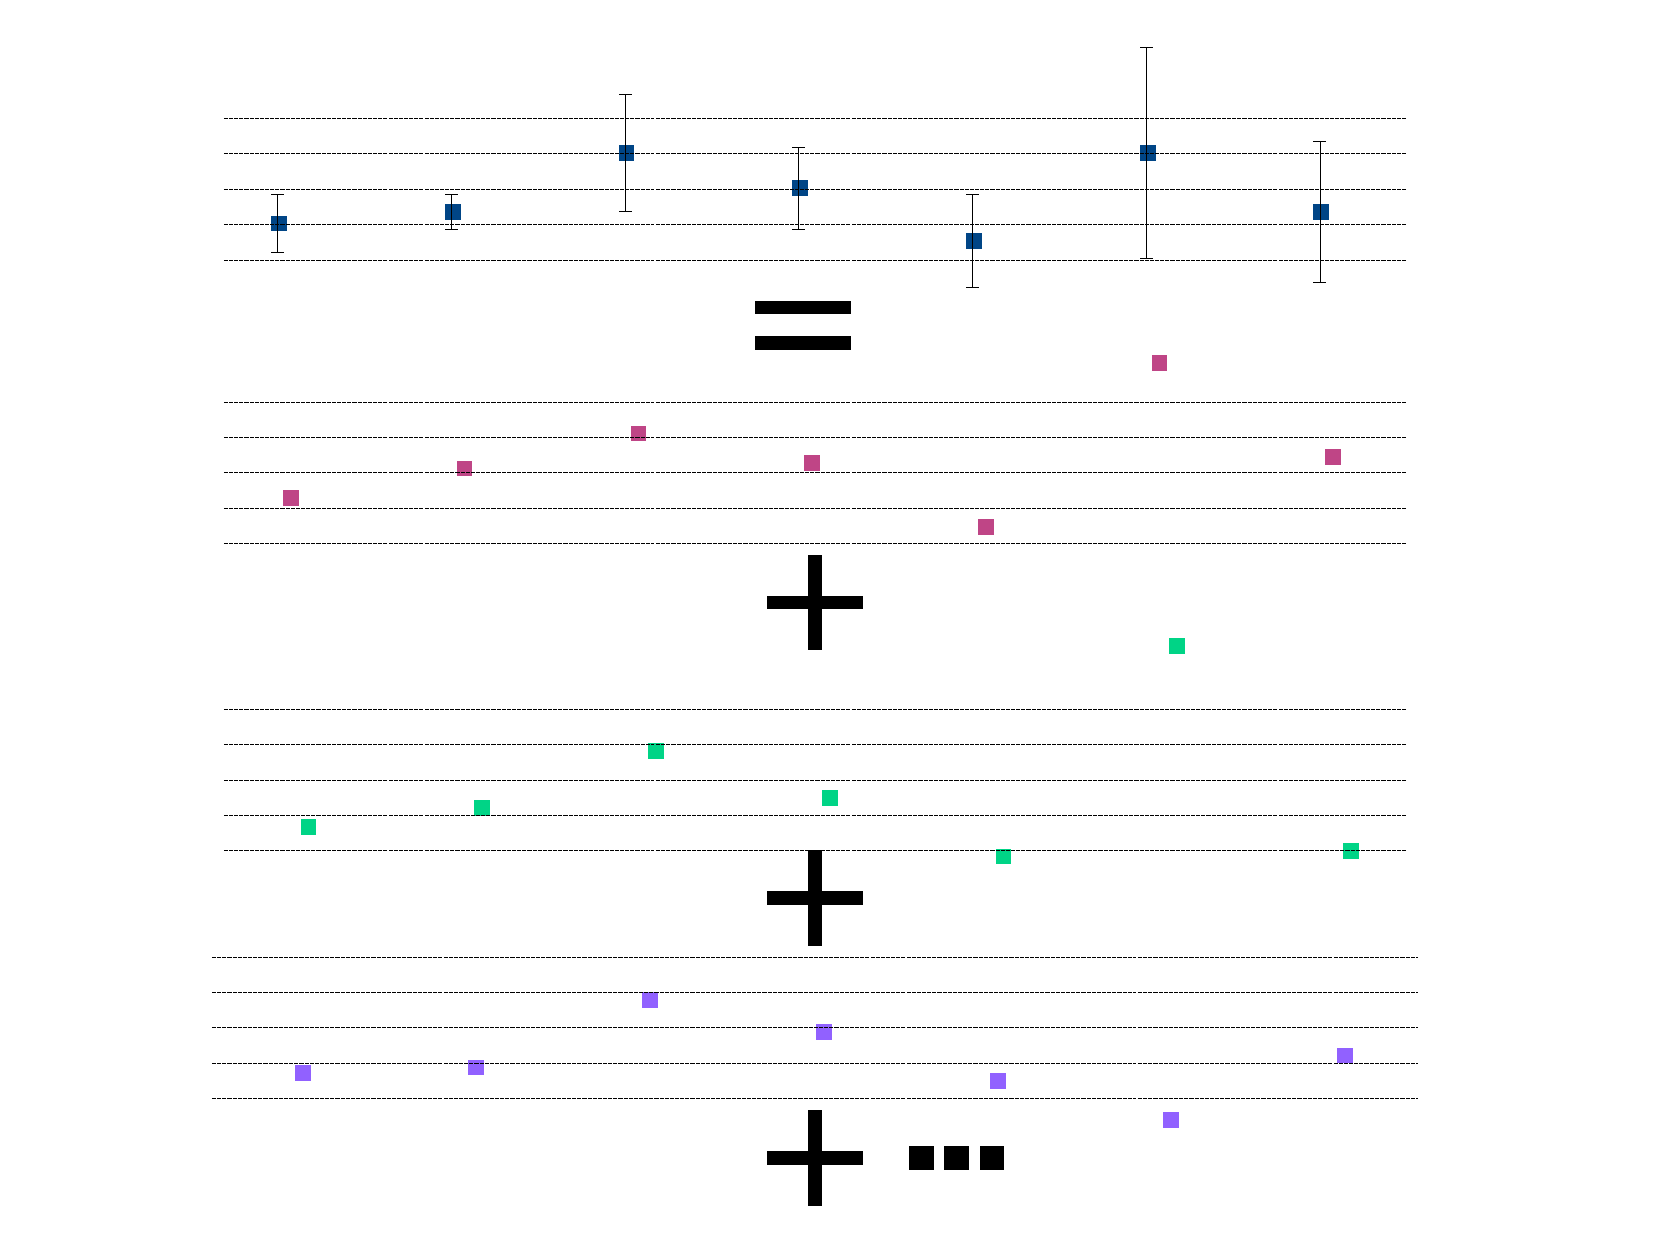
\includegraphics[width=0.7\textwidth]{background/monte_carlo.pdf}
\caption{Schematic of the generation of Monte Carlo replicas of pseudodata from data with uncertainties.}
\label{fig:MC}
\end{figure}
They are generated using Gaussian random numbers $n_a^{(k)}$ and $\hat{n}_p^{(k)}$:
\be
D^{(k)} = (D^0 + \sum_a n_a^{(k)} \sigma^a) \prod_m (1 + \hat{n}_m^{(k)}\sigma^p),
\ee
where $D_0$ is the (symmetrised) experimental data value, and $\sigma^a$ and $\sigma^m$ are the additive and multiplicative uncertainties discussed in Sec. \ref{sec:expuncs}. Explicitly, the pseudodata replicas satisfy the relations:
\be
\langle D_i^{(k)} \rangle = D_i^0; \qquad (\langle  D_i^{(k)} \rangle -D_i^0)(\langle  D_j^{(k)} \rangle-D_j^0) = C_{ij},
\ee
where the notation $\langle \cdot \rangle$ denotes the mean over replicas. Fig. \ref{fig:datarepchorus} shows the distribution of pseudodata for a single data point.

\begin{figure}
\centering
\includegraphics[width=0.7\textwidth]{background/datarepchorus.png}
\caption{Histogram of distribution of 100 pseudodata replicas for a single data point, normalised to $D^0$. The purple line is the mean value $\langle D^{(k)} \rangle$, which is equal to $D^0$ to arbitrary precision.}
\label{fig:datarepchorus}
\end{figure}
\begin{figure}
\centering
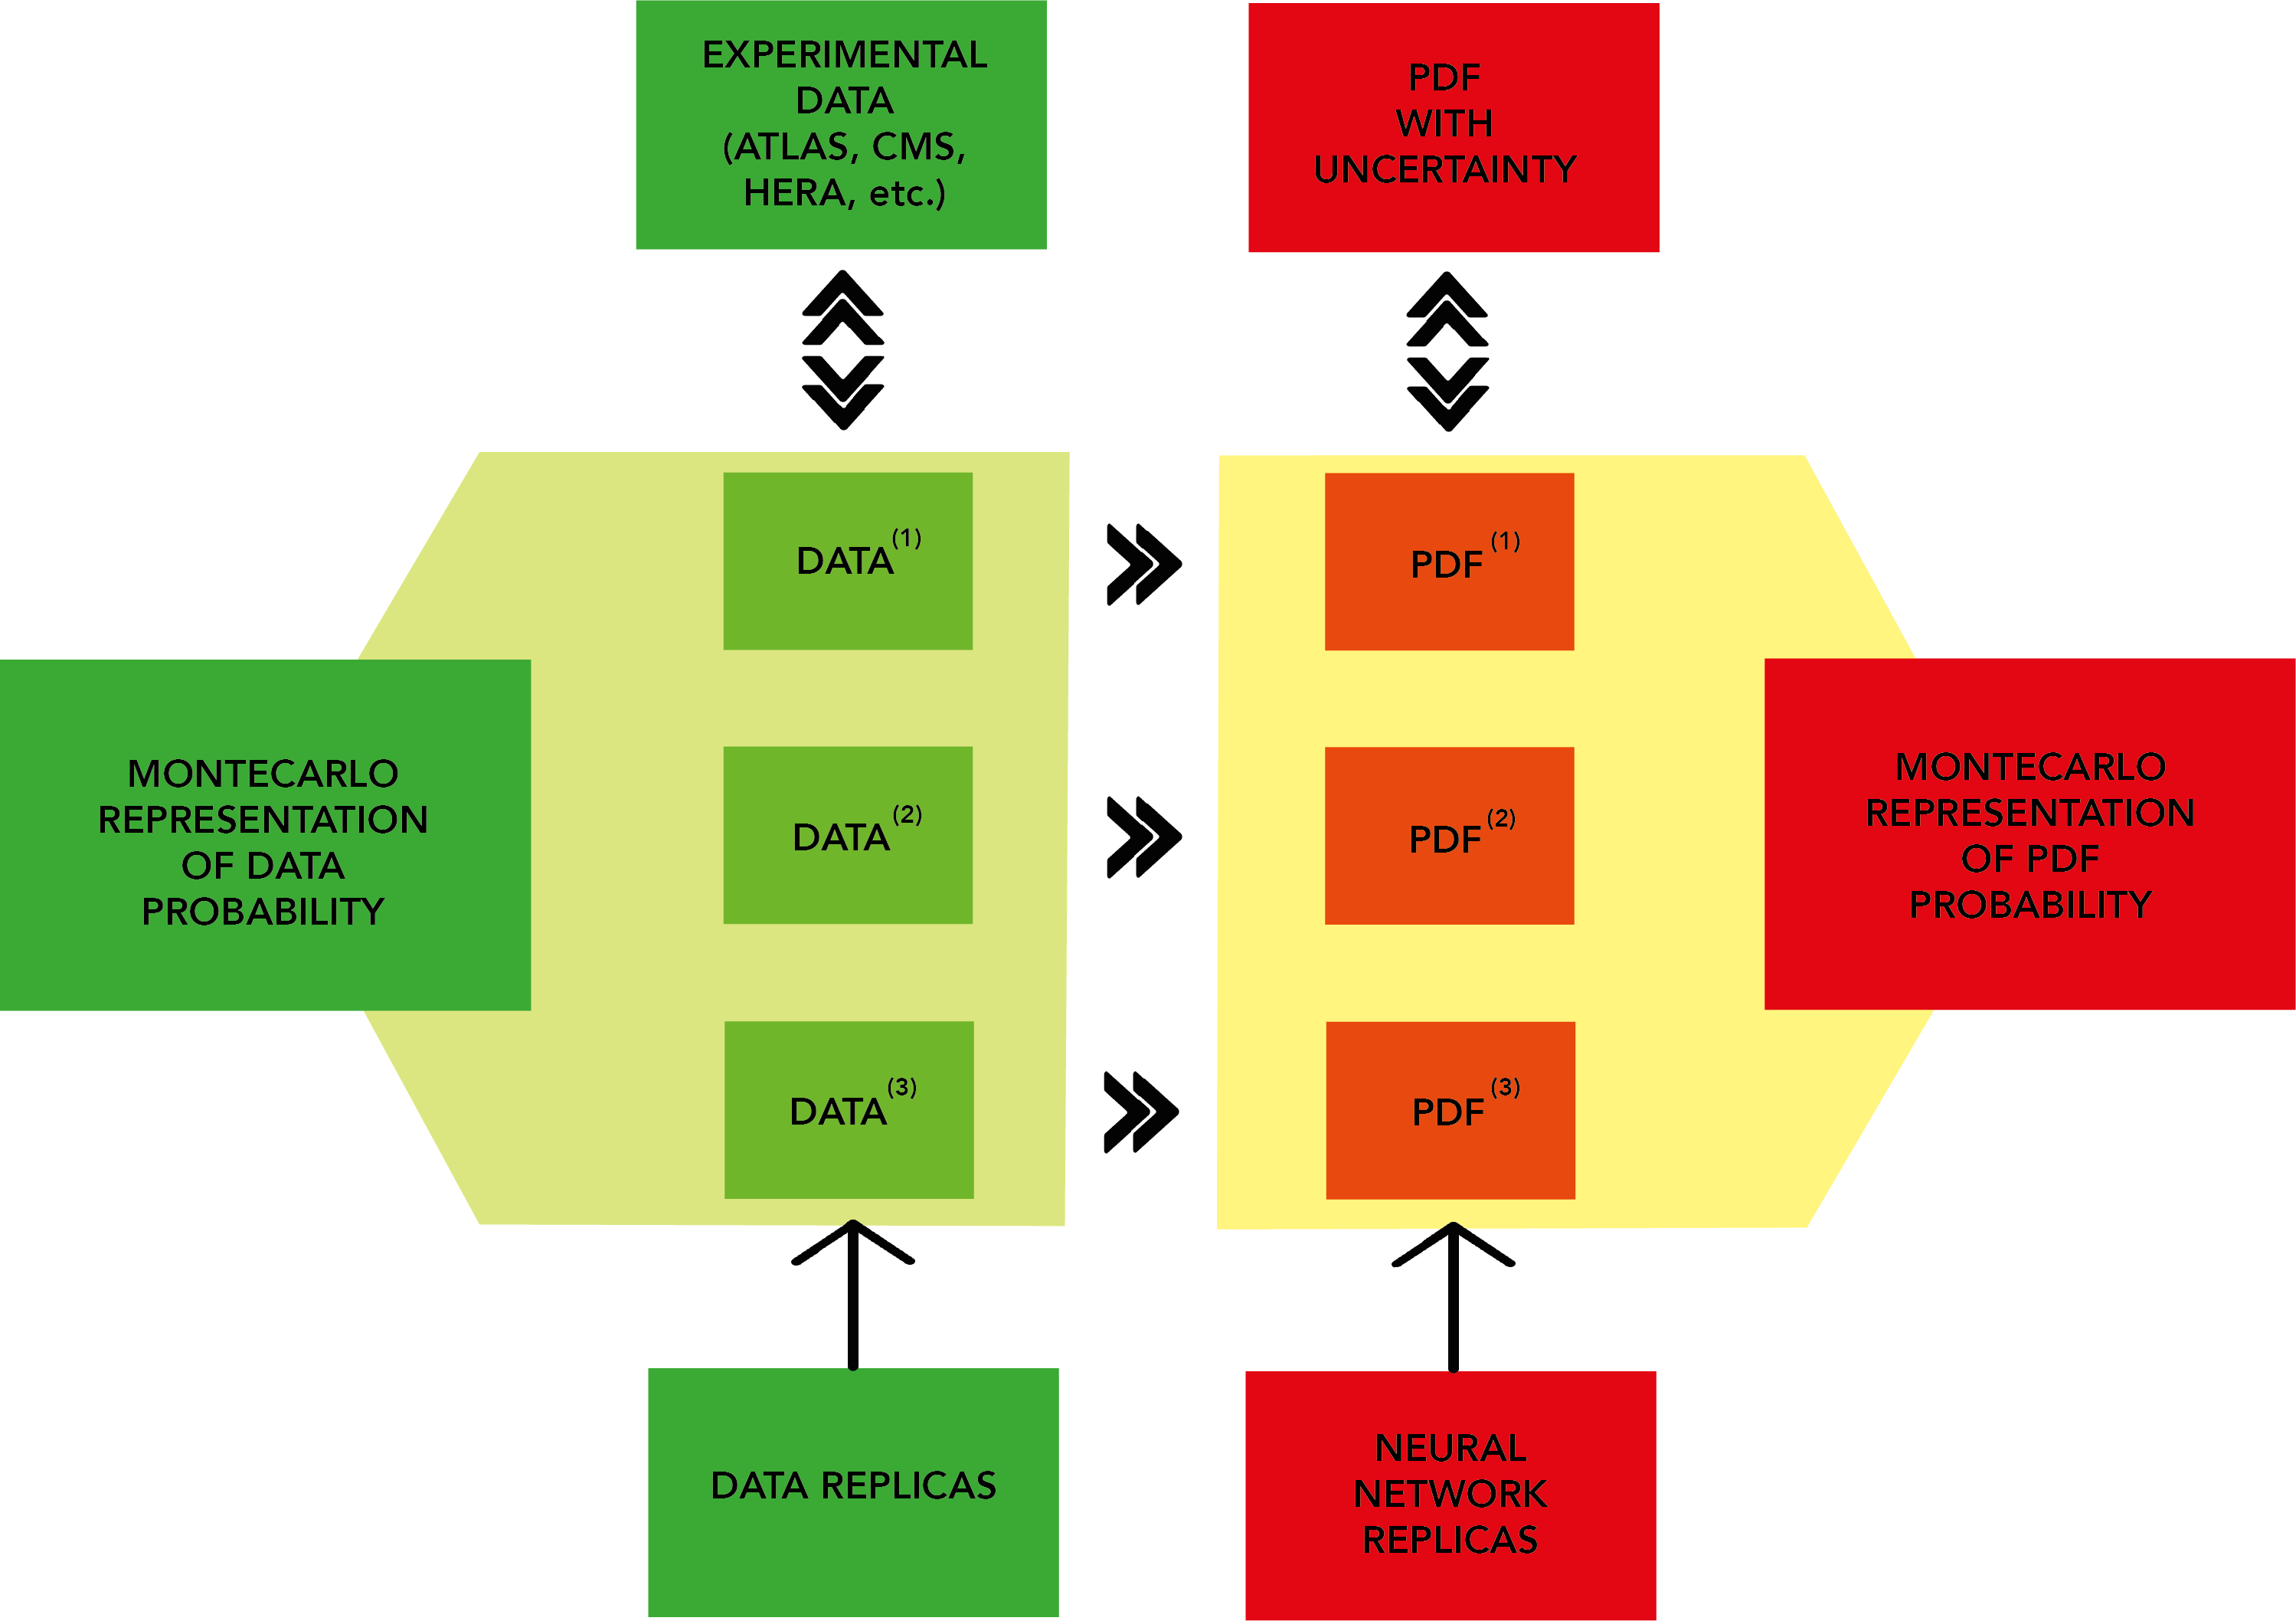
\includegraphics[width=0.8\textwidth]{background/generalstrategy.png}
\caption{NNPDF general strategy.}
\label{fig:generalstrategy}
\end{figure}
Once the pseudodata have been generated, each of these ($D^{(k)}$) is fitted separately to the theoretical predictions by minimising a target error function based on the $\chi^2$ (Eqn. \ref{eqn:chi2}), resulting in a PDF set of each flavour, $f_q^{(k)}$ (where $q$ runs over the fitted flavours: $g$, $u$, $d$, $s$, $c$, $\bar{u}$, $\bar{d}$, $\bar{s}$, $\bar{c}$). These act as a Monte Carlo parametrisation of the PDFs (for example, Fig. \ref{fig:replicas}).  This means that the PDFs and their errors can be extracted by taking the means and standard deviations over the ensemble. The final PDFs are made publicly available as downloadable files on the LHAPDF website \cite{lhapdf, Buckley:2014ana}. 

\begin{figure}
\centering
    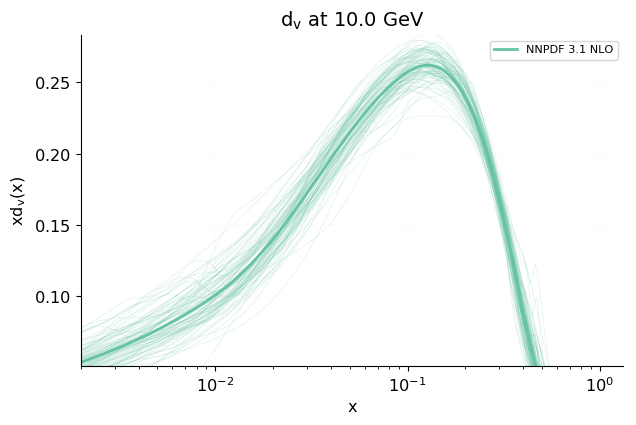
\includegraphics[width=0.7\textwidth]{background/Qs0_NNPDF31NLO_plot_pdfreplicas_d_v.png}
\caption{Monte Carlo replicas for the down valence quark PDF NNPDF3.1 at NLO. } \label{fig:replicas}
\end{figure}

\subsection{Neural Networks}

Inspired by how the brain processes information, in machine learning neural networks are a graph of connected nodes. They are trained by example, so
have the capability to learn a PDF's functional form given a set of data. The use of neural networks rather than specific functional forms allows us to avoid the theoretical bias which goes into selecting such a functional form. The layout, or ``architecture", consists
of input layers, hidden layers and output layers. Nodes can be either input nodes or activation nodes, the latter of which have an associated activation function which is applied to their output. Fig. \ref{fig:nn} depicts the architecture currently used by NNPDF. This is a ``2-5-3-1" archiecture, where the numbers refer to the number of nodes in each layer. It is a ``multilayer perceptron", meaning the graph is fully connected, and it is a feed-forward; information can only be passed in one direction through the layers (from 
input to output). The two inputs are $x$ and $\ln (1/x)$, and the output, $f$, is the PDF at the parametrisation scale, $Q_0$. In this network the output
of a node in the $l^{th}$ layer is given by
\beq
  \xi_i^{(l)} = g \bigg( \sum_j^{inputs} \omega_{ij}^{(l)} \xi_j^{(l-1)} + \theta_i^{(l)} \bigg)
\eeq
where the $\omega$s and $\theta$s are ``weights'' and ``thresholds''; parameters to be minimised
with respect to.  $g$ is an ``activation function'' which is set to
\beq
  g(z) =
\begin{cases}
 \frac{1}{1 + e^{-z}} &\text{for hidden layers}\\
  a &\text{for output layer}.
\end{cases}
\eeq
The choice of sigmoid activation function for the hidden layers allows sufficient non-linear freedom in the functional form, and the linear activation function for the output layer ensures the range of the PDFs is not restricted to [0,1].
\begin{figure}[H]
\centering
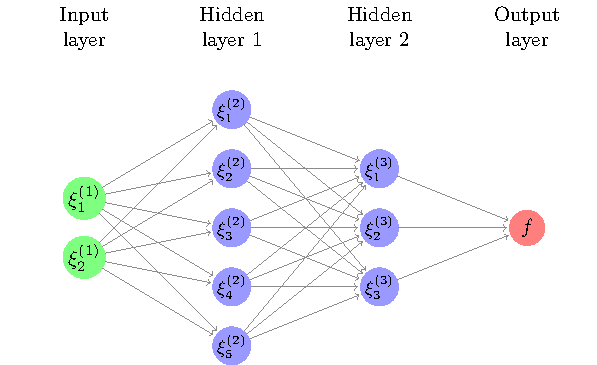
\includegraphics[width=\textwidth]{../diagrams/neuralnet.pdf}
\label{fig:nn}
\caption{Schematic depiction of the 2-5-3-1 architecture of an artificial neural network currently used by NNPDF. In the NNPDF methodology $\xi_1^{(1)}$ and $\xi_2^{(1)}$ are the variables $x$ and $\log x$ respectively.}
\end{figure}

The training of the neural networks is implemented using a ``genetic algorithm" (CMA-ES), so-called because of the introduction of mutation to the fitting parameters. This additional degree of randomness helps to avoid getting stuck in local minima. In practice, this involves ``mutating" some chosen fraction of the thresholds, $\theta$, by perturbing them at random.

\subsection{Parametrisation, preprocessing and postprocessing}
A scale of $Q=1.65$ $GeV$ is chosen to parametrise the PDFs at, and then they can be determined at any other scale by evolution using the DGLAP equations (Eqn. \ref{eqn:DGLAP}). The PDFs are fitted parametrised in a ``fitting basis", to help convergence \cite{Ball:2014uwa}, defined:
\begin{itemize}
\item $g$;
\item $\Sigma \equiv \sum_{u,d,s} q_i + \bar{q}_i$;
\item $T_3 \equiv u - d$;
\item $T_8 \equiv u + d - 2s$;
\item $V \equiv \sum_{u, d, s} q_i - \bar{q}_i$;
\item $V_3 \equiv \bar{u} - \bar{d}$;
\item $V_8 \equiv \bar{u} - \bar{d} - 2 \bar{s}$;
\item $c$.
\end{itemize}
Since the form of the neural networks ($N_i(x)$) is determined by training on experimental data, the output is not meaningful outwith the data region. The functional form of the PDFs in this so-called ``extrapolation region" is in practice fixed through enforcement of the known high and low $x$ behaviour via ``preprocessing"; the PDFs are parametrised as:
\beq
  f_i(x) = A_i x^{-\alpha_i} (1-x)^{\beta_i} N_i(x).
\eeq
$A_i$ are normalisation coefficients set by the sum rules and fixed at each iteration of the fit. The powers $\alpha_i$ and $\beta_i$ are fitted parameters determined by iteration from one fit to the next. This preprocessing has the effect that the PDFs approach 0 at large $x$, and generally grow at small $x$. This is because the probability of the existence of a parton is generally small at high $x$ and larger with decreasing $x$ outwith the data region.

Postprocessing is also applied to the PDF replicas to remove those which don't satisfy certain quality conditions. That is, where the target error function or arc-length of the replica is more than four standard deviations outwith the mean, or where the positivity of the resulting cross-sections is not satisfactorily maintained. 

\subsection{Cross validation}
Neural networks are effective at learning the functional form underlying data. Sometimes they can be ``too effective", picking up not just the underlying law but also the noise. This is known as ``overlearning" (see Fig. \ref{fig:overlearning} for an example).

\begin{figure}[H]
\centering
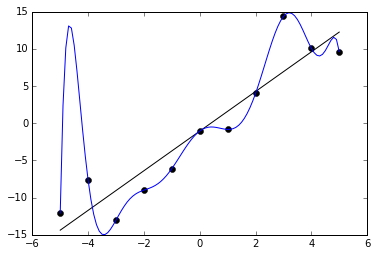
\includegraphics[width=0.6\textwidth]{background/overfitteddata.png}
\label{fig:overlearning}
\caption{Overlearning: the data points (black dots) fluctuate around the linear underlying law (black line), but the neural network continues to minimise the error function until it passes through every data point (blue curve), fitting the noise in the data.}
\end{figure}

To circumvent this problem, the data is split into a training and a validation set. The training data is used to optimise the neural network, and the validation data is used to test the network output, in a process known as ``cross validation". As training epochs elapse, the target error function compared to both the training and validation data should decrease as the network learns the underlying law. At some point, however, the network will begin to learn the noise in the training data, at which point the training error function will continue to decrease, but the validation error function will stop decreasing and start to increase again. The optimum fit is determined using the ``lookback" method, where after training the model corresponding to the minimum in the validation error function is selected.

\begin{figure}[H]
\centering
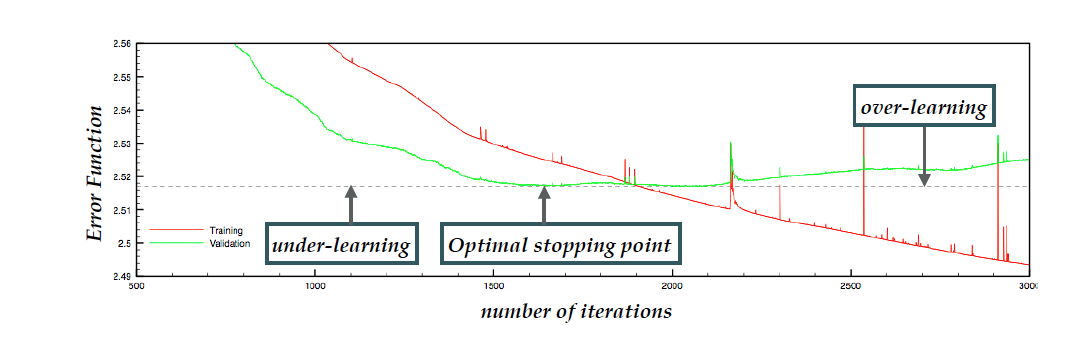
\includegraphics[width=\textwidth]{background/crossvalidation.png}
\label{fig:crossvalidation}
\caption{Cross validation with the lookback method.}
\end{figure}

\begin{figure}[H]
\centering
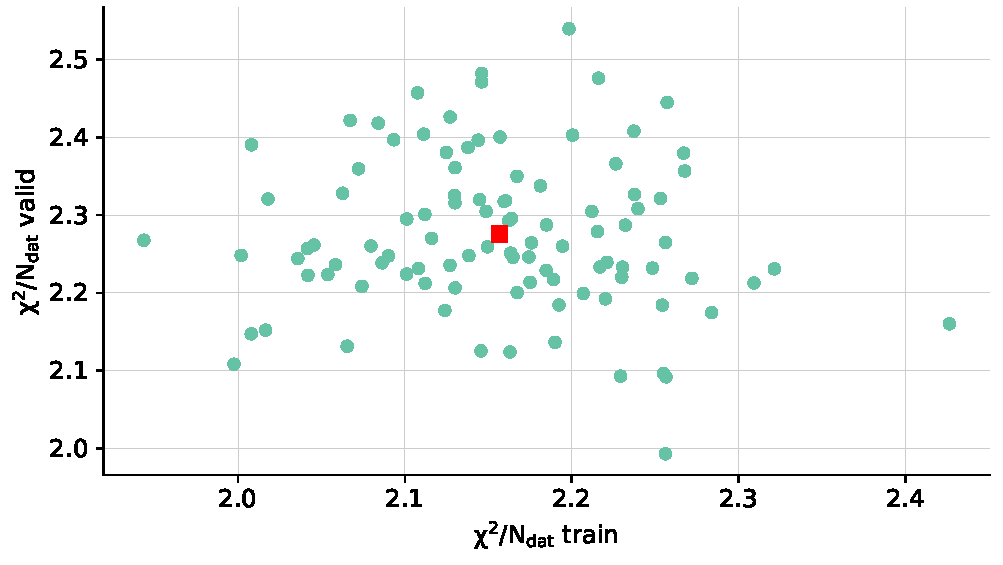
\includegraphics[width=\textwidth]{background/trvalchi2.pdf}
\label{fig:crossvalidation}
\caption{Comparing the training and validation $\chi^2$s for the 100 replicas (green circles) of a PDF fit. The red square gives the average.}
\end{figure}
